\section{LLT Polynomials}
\label{sec:llt}

The \textit{LLT polynomials} were first introduced by Lascoux, Leclerc
and Thibon for the purpose of generalizing products of Schur
functions.  It was defined as tilings of $k$-ribbons weighted by
$q$-counting a \textit{spin} parameter.  Spin was quite difficult to
work with to the extend that the symmetry of LLT's were conjectured in
the original paper!  Using geometric techniques, Grojnowski and Haiman
introduced a \textit{inversion} statistics on arbitrary tuples of skew
shaps and proved that such polynomials were indeed the LLT obtaining a
simpler way to work with these polynomials.  Haglund, Haiman and
Loehr, in their study of a combinatorial formula for MacDonald
polynomials, obtained an elementary proof of its symmetry using an
inductive argument.

\subsection{Definition}
\label{sec:definition}

Let $\nu = (\nu^{(1)}, \dots, \nu^{(k)})$ be a list of skew shapes.  A
\textit{semi-standard Young tableaux of shape $\nu$} is an element of
the set
\[
  SSYT(\nu) = SSYT(\nu^{(1)}) \times \cdots \times SSYT(\nu^{(k)}).
\]
The \textit{inversion} statistics on a tableau $T \in SSYT(\nu)$ is
defined as follows: A pair of (labelled) cells $(\square,\square')$ contributes
$1$ to $inv(T)$ if and only if $T^{(i)}(\square) > T^{(j)}(\square')$ and either
\begin{itemize}
\item \textbf{(D1)} $i < j$ and $c(\square) = c(\square')$, or
\item \textbf{(D2)} $i > j$ and $c(\square) = c(\square') + 1$.
\end{itemize}

\begin{figure}[H]
  \centering
  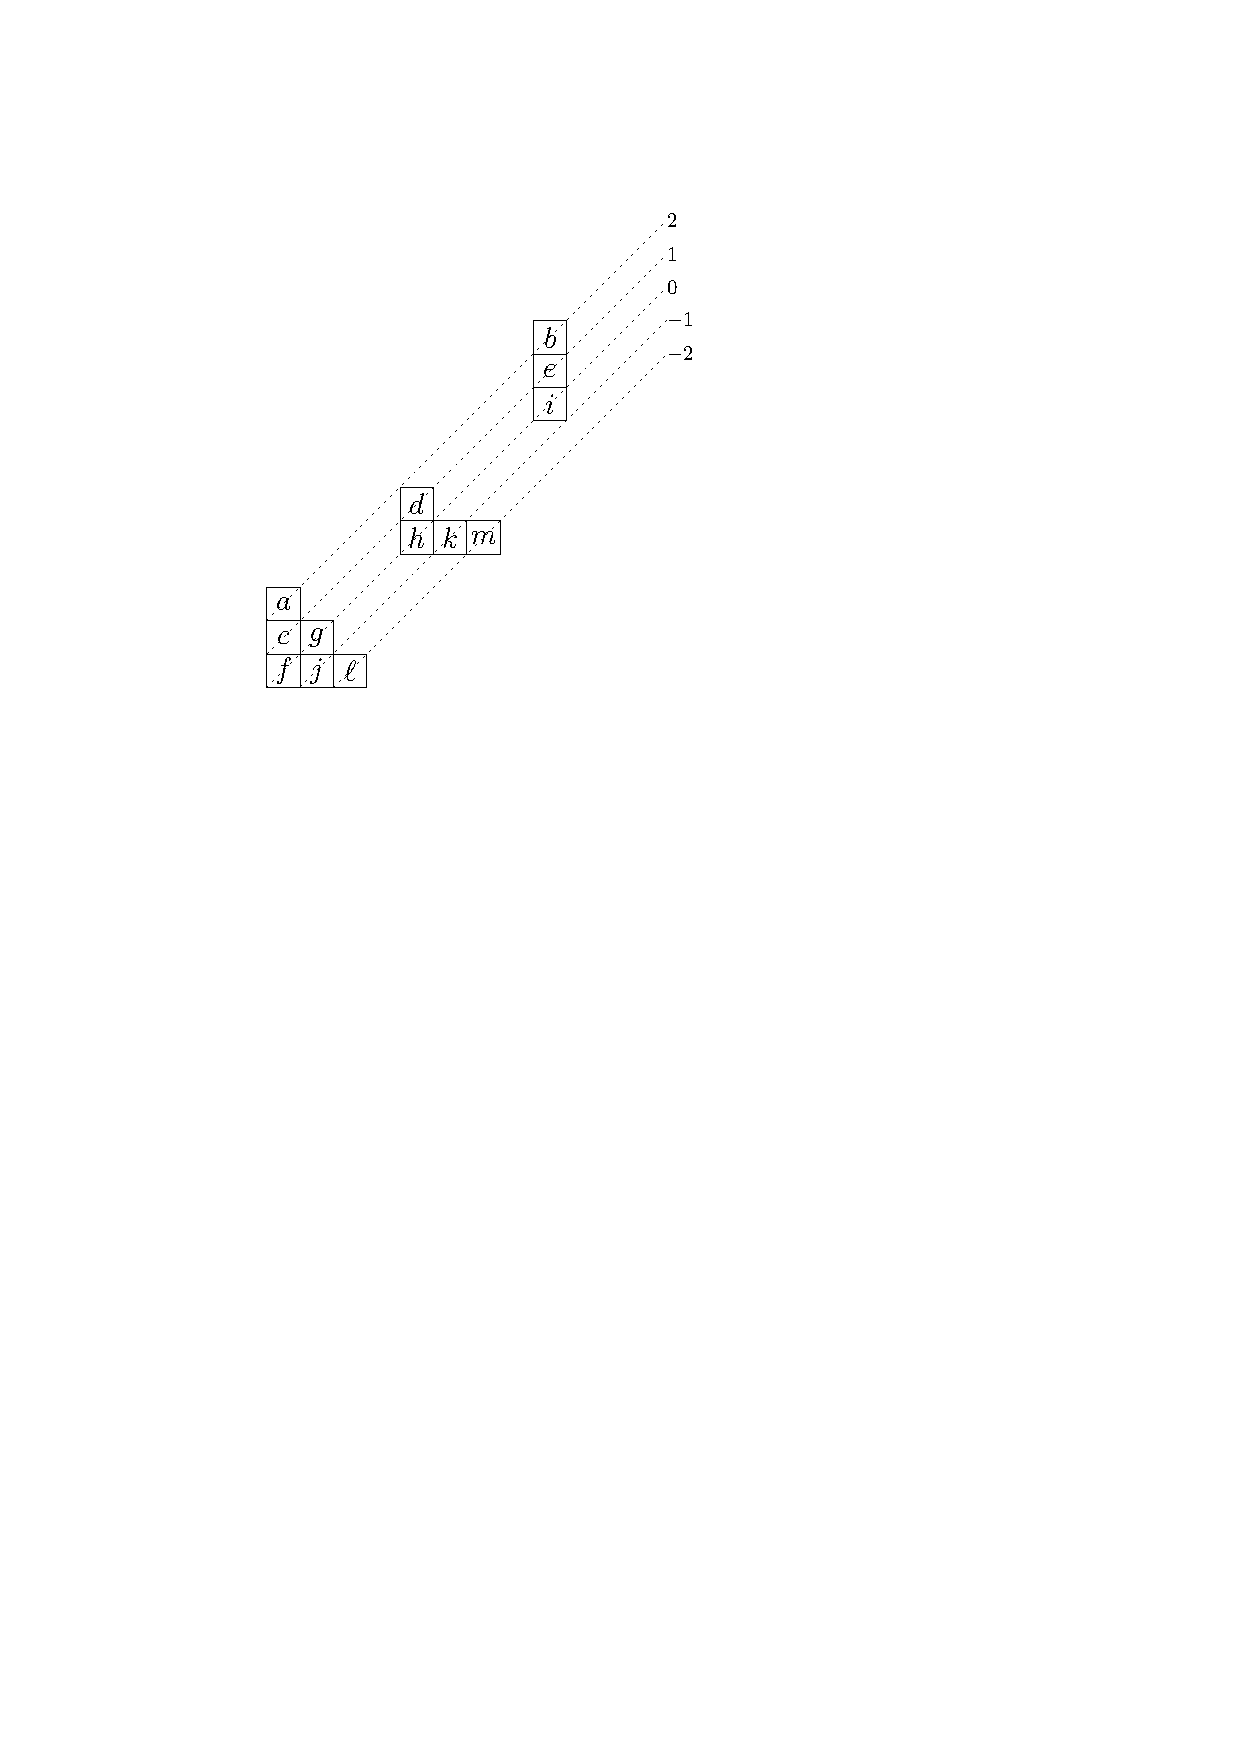
\includegraphics[scale=0.75]{sym/example1}
  \caption{An LLT tableau}
\end{figure}

The LLT polynomial indexed by $\nu$ is defined to be
\[
  G_{\nu}(x_{1},\dots,x_{n};q) = \sum_{T \in SSYT(\nu)} q^{inv(T)} \prod_{\square \in \nu}
  x_{T(\square)}.
\]
When $q=1$, we have $G(x_{1}, \dots, x_{n}; 1) = s_{\nu^{(1)}} \cdots s_{\nu^{(k)}}$.

There is a trivial way to represent products of LLTs. To multiply two
LLT polynomials $G_{\nu}$ and $G_{\rho}$, we simply ``stack'' $\nu$ on top of
$\rho$ such that the lowest cell in the $\nu$ is at least $2$ diagonals
away from the highest cell in $\rho$.  To factor an LLT, we simply
``cut'' along empty diagonals.

\subsection{Symmetry Proof}
\label{sec:symmetry}

We start with a series of reductions.

\begin{enumerate}[label=\textbf{(R\arabic*)}]
\item It suffices to prove that $G_{\nu}(x_{1},x_{2};q)$ is symmetric.

  Let $\nu = (\nu^{(1)}, \dots, \nu^{(k)})$ be skew shapes.  Note
  \[
    SSYT(\nu) = \bigcup_{\rho \subseteq \nu} \bigg\{ T \in SSYT(\nu) : T^{-1}(\{i,i+1\}) = \rho \bigg\}
  \]
  is a disjoint union.  Then for every $\rho \subseteq \nu$ and
  $S: \nu\setminus\rho \to \mathbb{N} \setminus \{i,i+1\}$ with
  $S \cup T \in SSYT(\nu)$ for some $T \in SSYT(\rho)$, there exists some
  $i(\nu,\rho,S)$, independent of its completion to SSYT, such that
  \begin{align*}
    G_{\nu}(x_{1}, \dots, x_{n}; q)
    &= \sum_{\rho \subseteq \nu} \sum_{\substack{T \in SSYT(\nu)\\T^{-1}(\{i,i+1\}) = \rho}}
      q^{inv(T)} x^{T|_{\nu \setminus \rho}} x^{T|_{\rho}} \\
    &= \sum_{\rho \subseteq \nu} \left( \sum_{\substack{T \in SSYT(\rho)\\T(\rho)\subseteq\{i,i+1\}}} q^{inv(T)}
    x^{T}\right) \left( \sum_{S} q^{i(\nu,\rho,S)} x^{S} \right) \\
    &= \sum_{\rho \subseteq \nu} G_{\rho}(x_{i},x_{i+1}; q) \left( \sum_{S} q^{i(\nu,\rho,S)} x^{S} \right).
  \end{align*}

\item We can assume $\nu$ consists of horizontal strips.

  We can assume each $\nu^{(j)}$ is a disconnected union of $2$-row skew
  shapes otherwise $G_{\nu}(x_{1},x_{2}; q) = 0$.  Take a closer look at
  the contribution to $inv$ for each vertical domino.
  \begin{figure}[H]
    \centering
    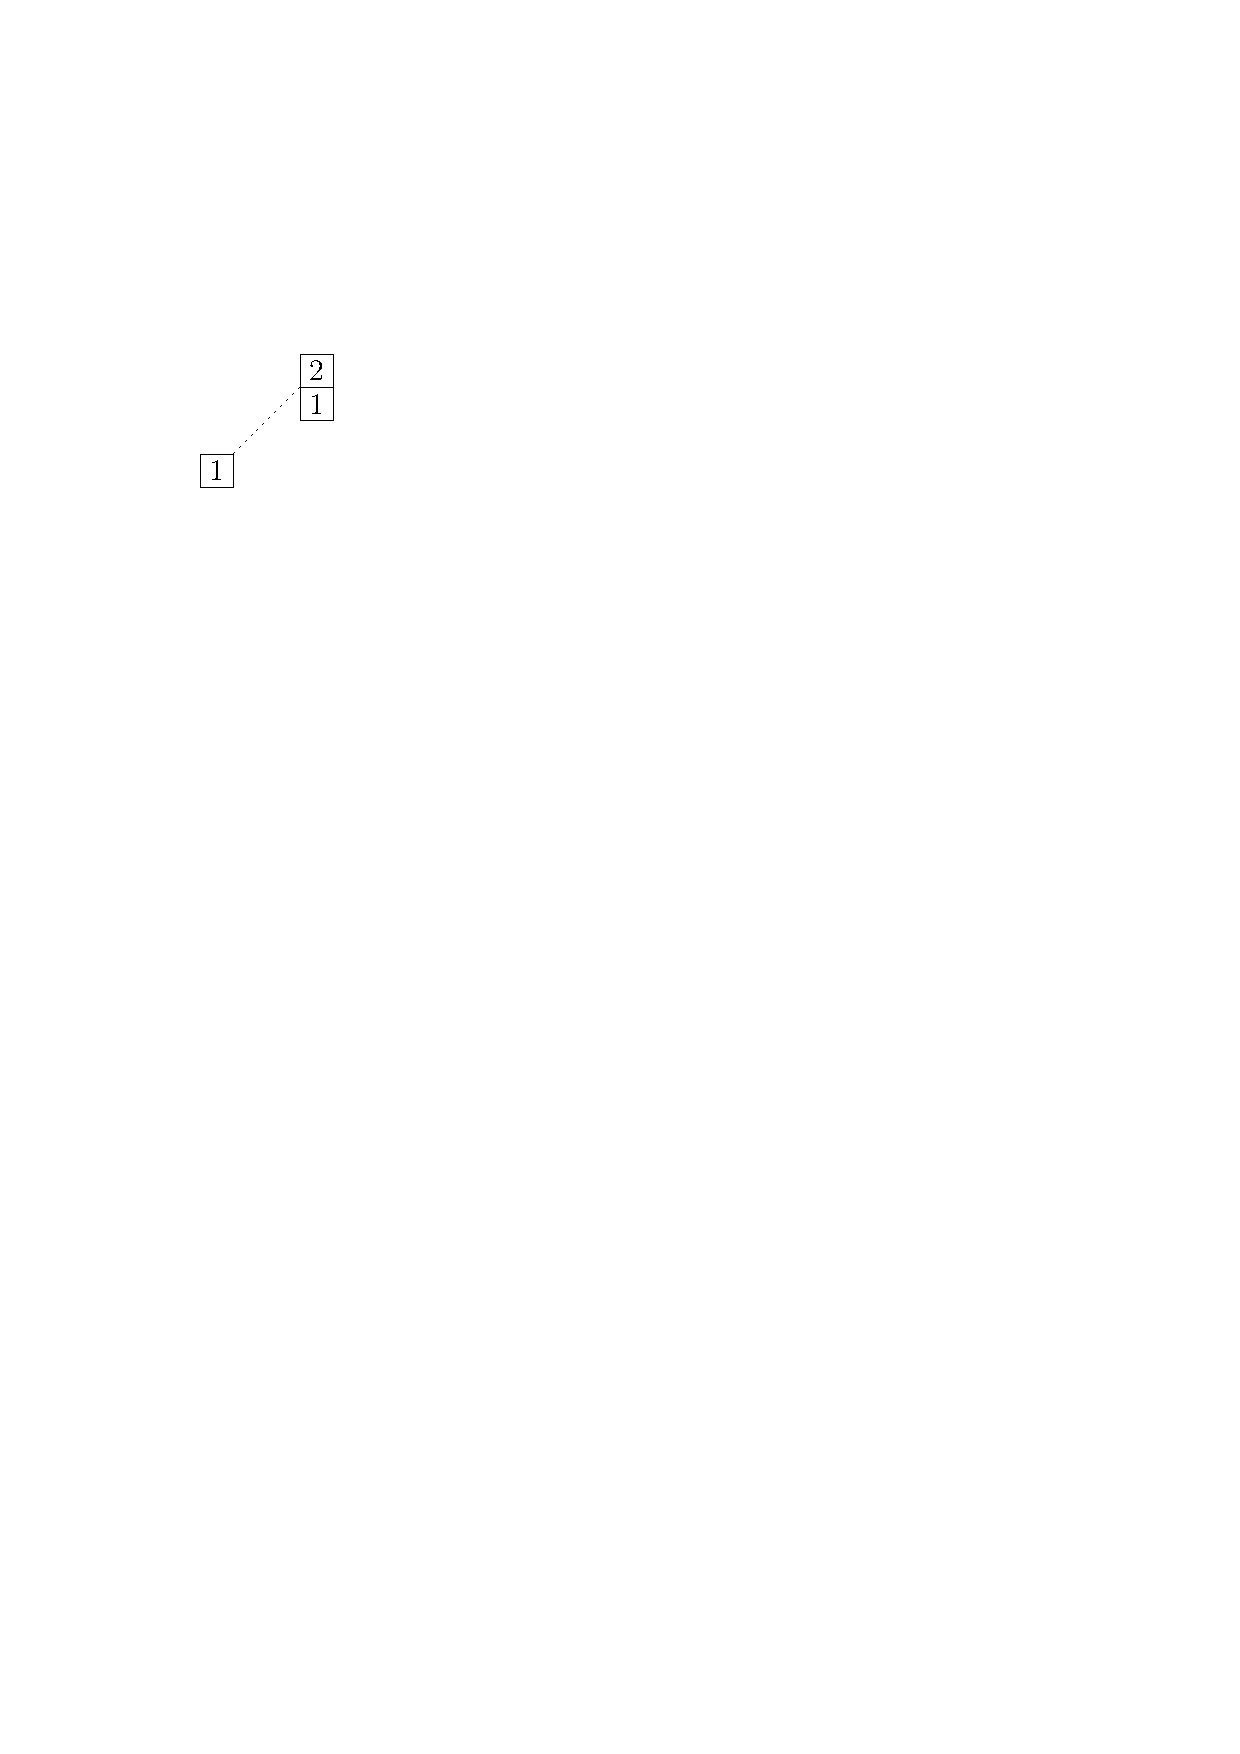
\includegraphics{sym/R2-1}
    \quad
    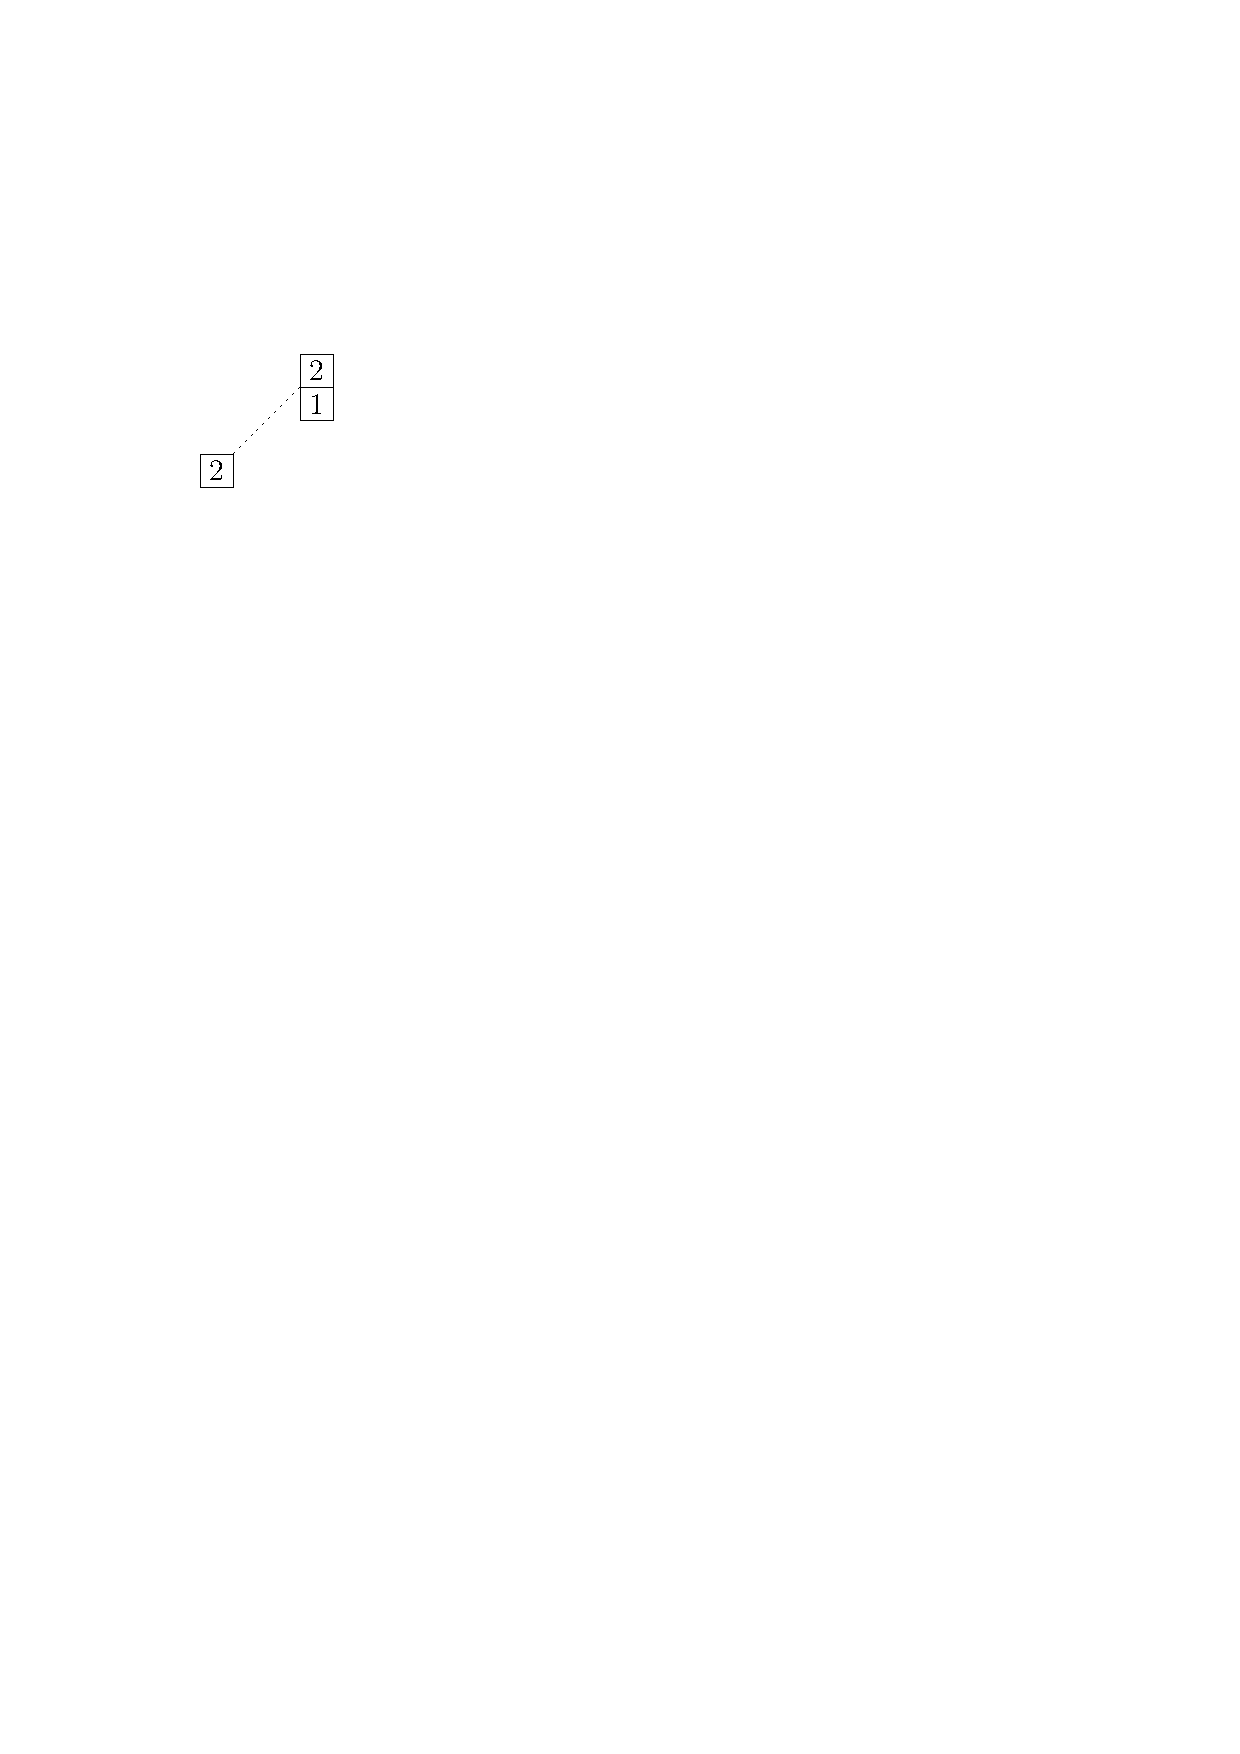
\includegraphics{sym/R2-2}
    \quad
    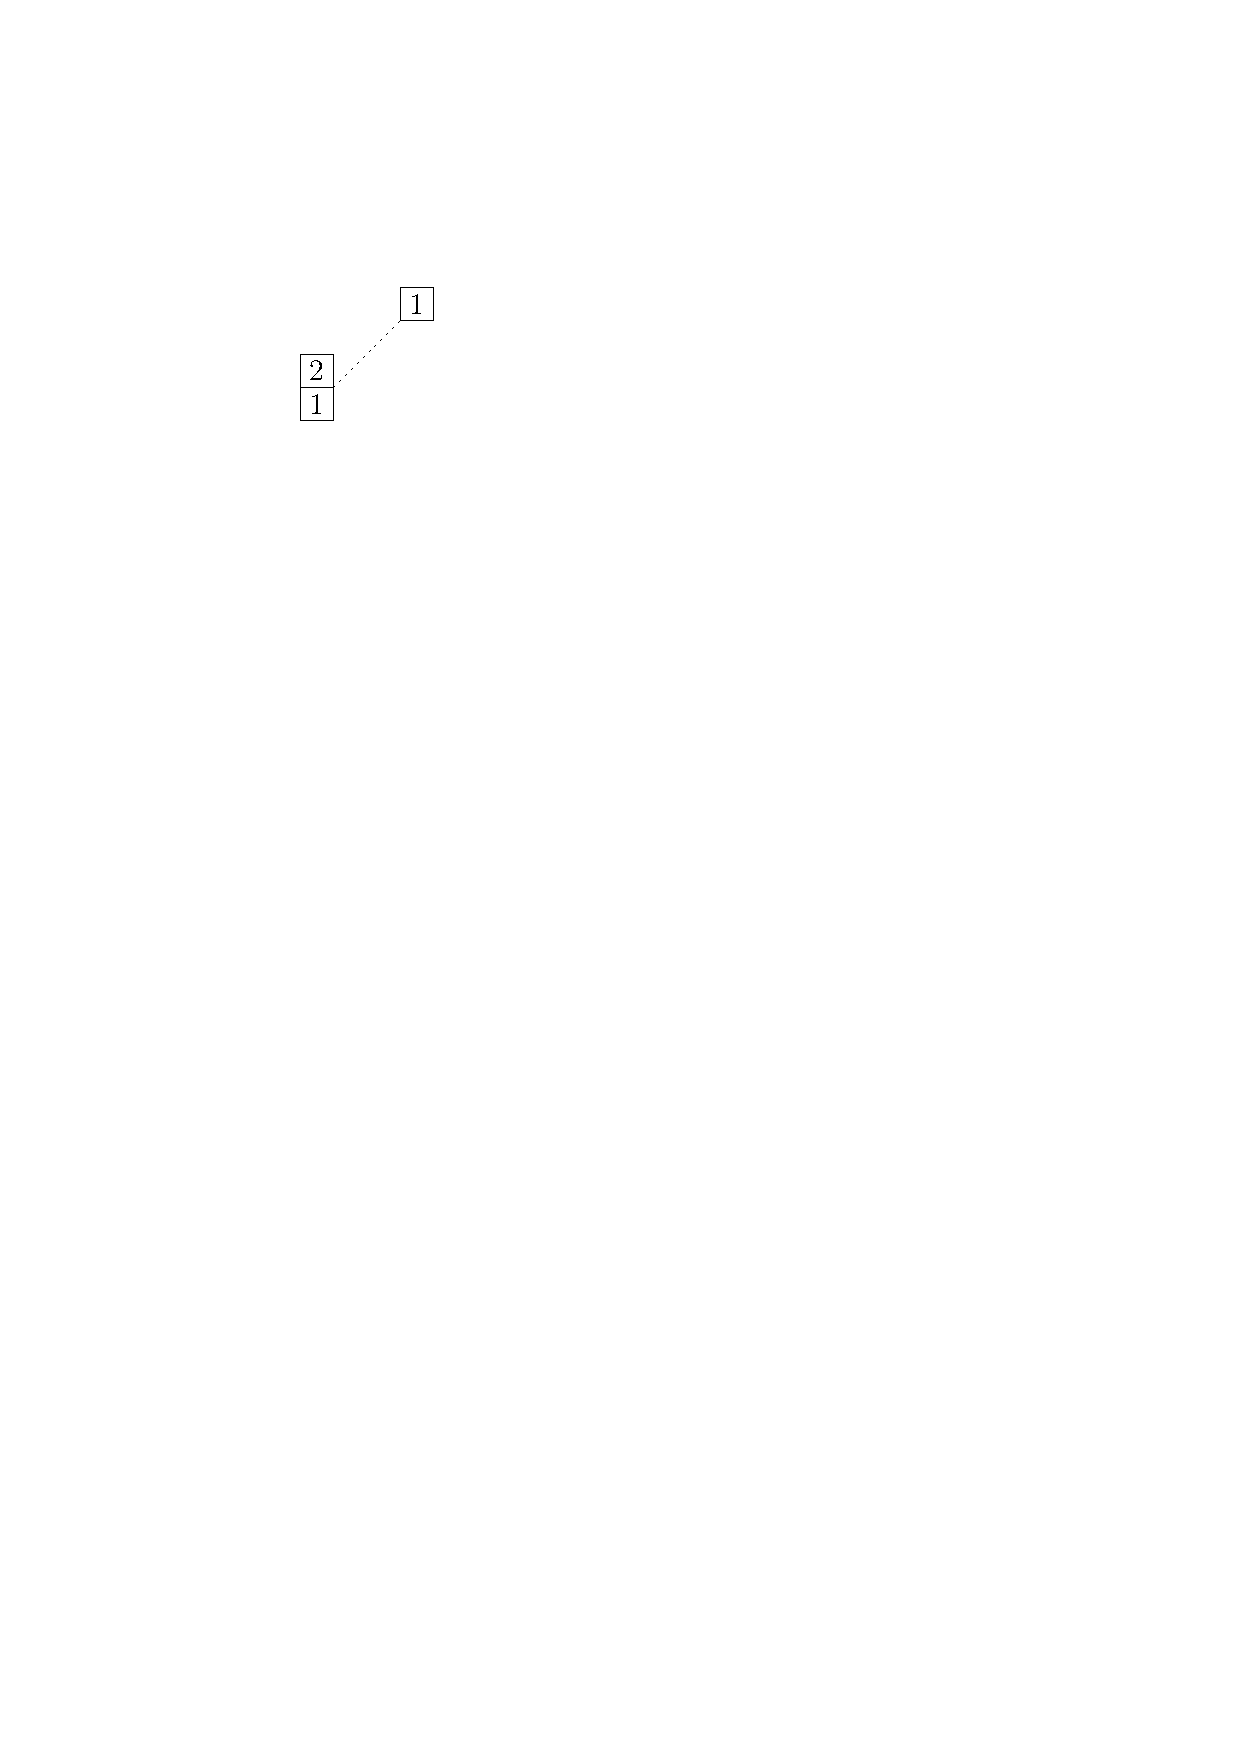
\includegraphics{sym/R2-7}
    \quad
    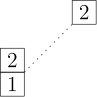
\includegraphics{sym/R2-8}
    \caption{No contribution to $inv$.}
  \end{figure}

  \begin{figure}[H]
    \centering
    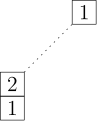
\includegraphics{sym/R2-3}
    \quad
    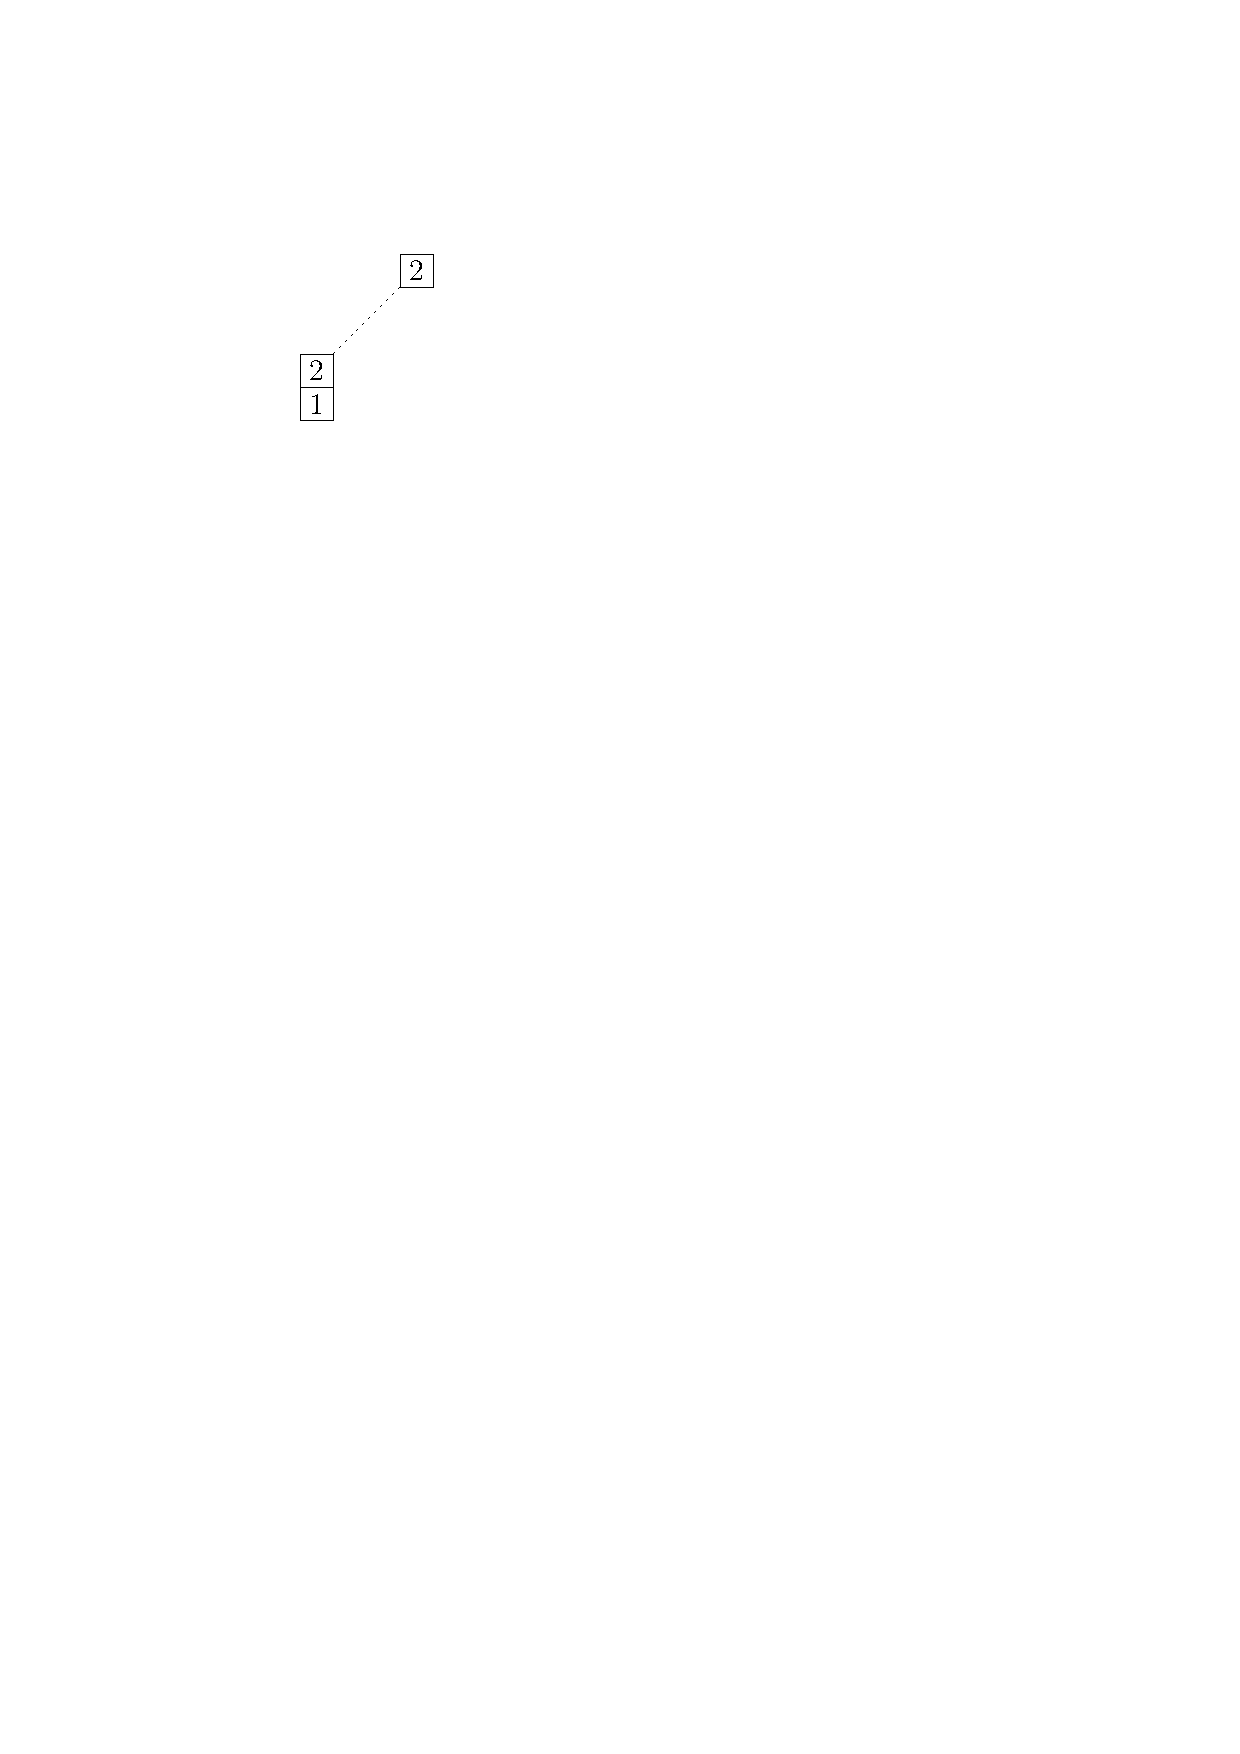
\includegraphics{sym/R2-4}
    \quad
    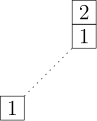
\includegraphics{sym/R2-5}
    \quad
    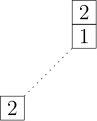
\includegraphics{sym/R2-6}
    \caption{Contributes $1$ to $inv$.}
  \end{figure}

  Let $\rho$ be the set of vertical dominoes in $\nu$.  Then
  $\nu \setminus \rho$ is a horizontal strip.  Remember that we are in French
  notation.  We can put anything we want to the left of $2$ and to the
  right of $1$.  So every $SSYT(\nu \setminus \rho)$ can be obtained as
  $T|_{\nu \setminus \rho}$ for some $T \in SSYT(\nu)$.  Then for some
  $h(\nu)$, independent of choice of tableaux, we have
  \begin{align*}
    G_{\nu}(x_{1},x_{2}; q)
    &= q^{h(\nu)}(x_{1}x_{2})^{|\rho|/2} \sum_{T \in SSYT(\nu \setminus \rho)} q^{inv(T)} x^{T} \\
    &= q^{h(\nu)}(x_{1}x_{2})^{|\rho|/2} G_{\nu \setminus \rho}(x_{1},x_{2}; q).
  \end{align*}

\item We can also assume $\nu$ consists of horizontal strips.

  Using superization techniques, there exists some $m \ge 0$ such that
  \[
    G_{\nu'}(x_{1},\dots,x_{n}; q) = q^{m} \omega G_{\nu}(x_{1}, \dots, x_{n}; 1/q),
  \]
  where $\nu' = (\nu^{(k)'}, \dots, \nu^{(1)'})$.  We will come back to this
  later.

  It is difficult to finish the symmetry proof from here by a direct
  combinatorial argument analogous to the Bender-Knuth involution
  without using reciprocity.

\item We can assume $\nu$ is unicellular.

  Suppose $|\nu| = n$.  By the previous two reductions, we can assume
  $\nu$ is both a horizontal strip and a vertical strip.  This is only
  possible when $\nu$ consists of disconnected cells.  So
  $SSYT(\nu) = \{1,2\}^{n}$ since column and row restrictions on tableaux
  are void.  This means $\nu$ is unicellular which means we can simply
  think of $\nu$ as a list of contents
  $c(\square_{1}), \dots, c(\square_{n})$ in content reading order.  But we will
  represent them visually in a uniform way.

  Fix any cell $\square \in \nu^{(j)}$.  Since $\nu^{(j)}$ is a skew shape,
  another cell $\square' \in \nu^{(j)}$ appearing above $\square$ must also appear to
  its left (remember we are French for now).  Moving cells along the
  diagonal does not affect the $inv$-statistics on $SSYT(\nu)$.  Hence
  we can assume all cells of $\nu$ lies on the same reverse diagonal.
  \begin{figure}[H]
    \centering
    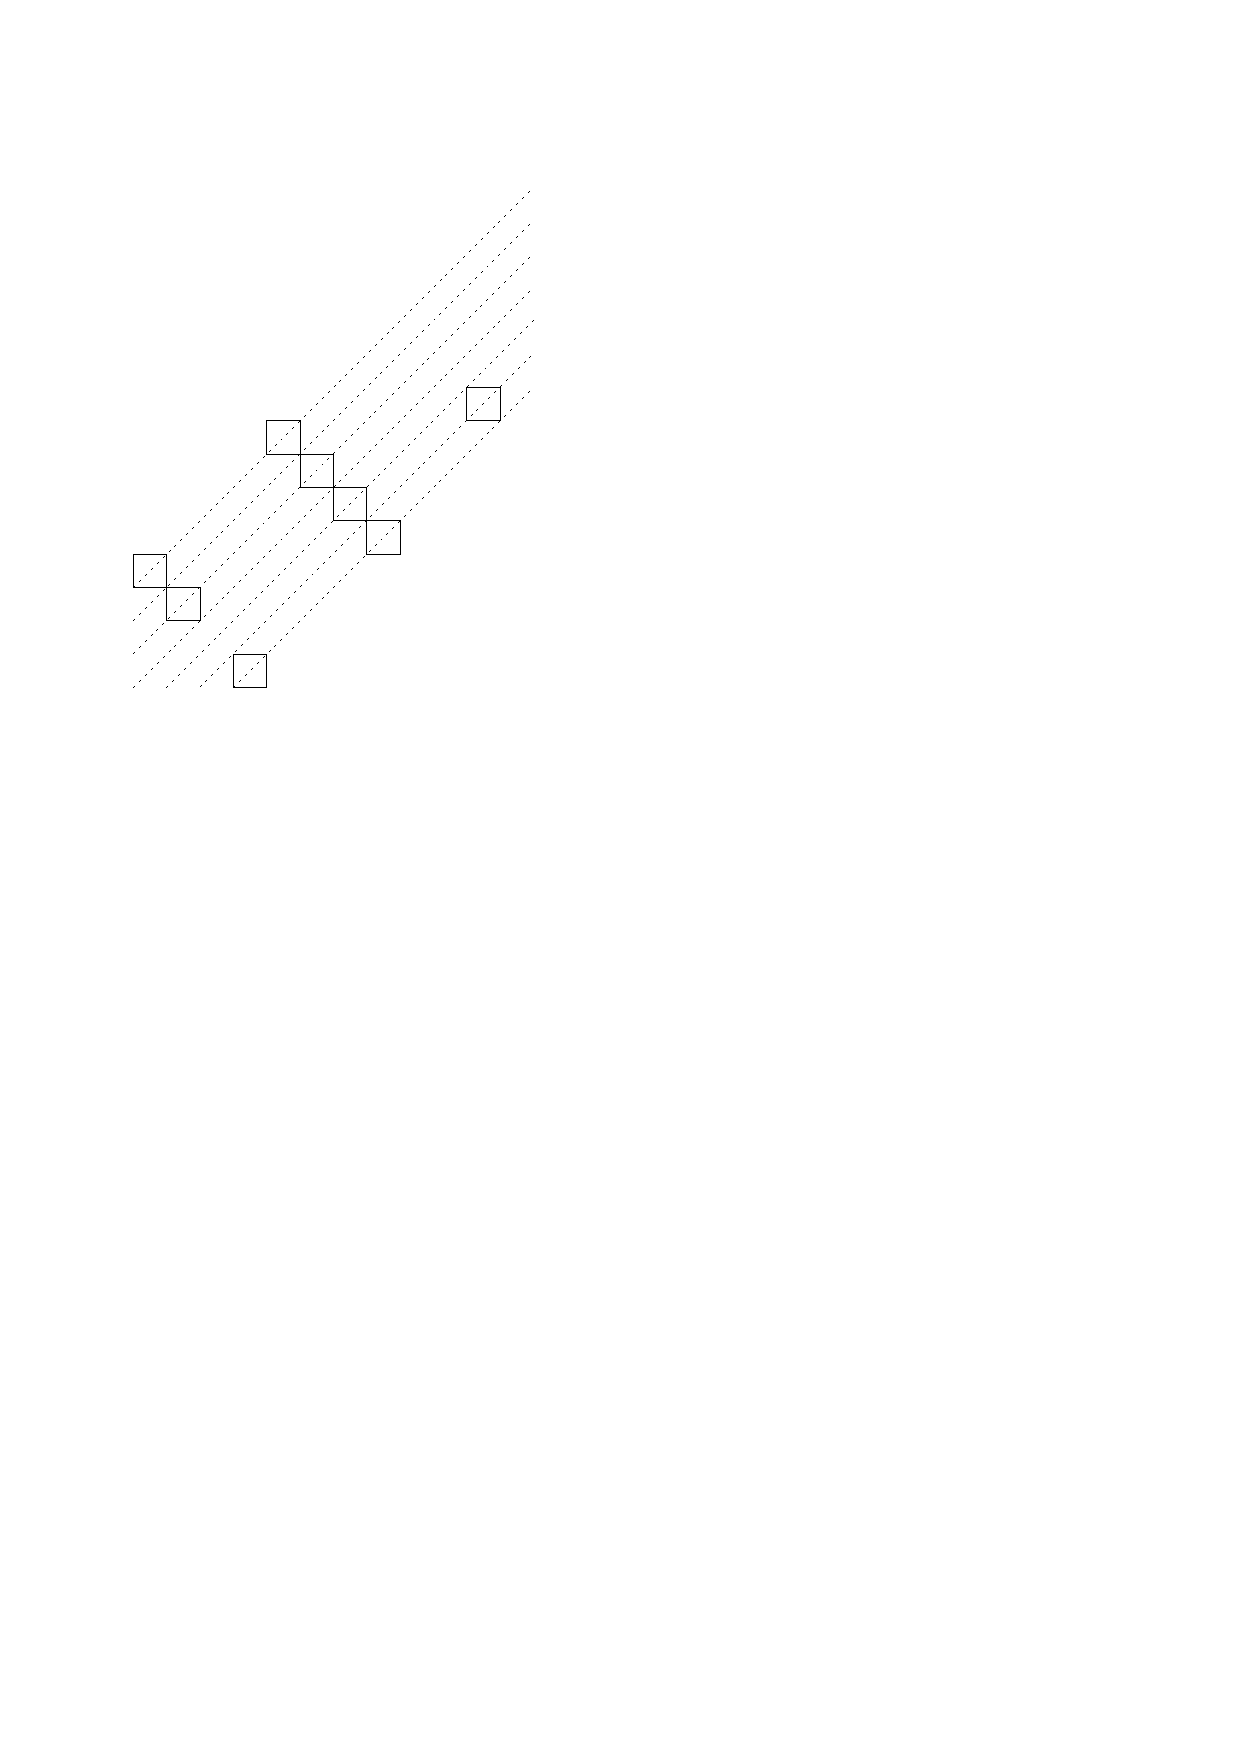
\includegraphics[scale=0.75]{sym/R4}
  \end{figure}
\end{enumerate}

Let $\beta = (\beta^{(1)}, \dots, \beta^{(k)})$ with $|\beta| = n$. Let
$\square_{n-r}$ be the first cell in content reading order such that
$(\square_{n-r}, \square_{n})$ could potentially contribute to $inv$.  Hence
$n-r$ is the index of the first cell appearing to the right of
$\square_{n}$ and in diagonal $c(\square_{n})-1$.

We proceed by double induction, first on $n \ge 1$, then on $r \ge 0$.
The result is trivial when $n=1$.  When $r = 0$, then $\square$ never
contribute to $inv$ so we simply factor (effectively deleting the cell
$\square_{n}$)
$G_{\beta}(x_{1},x_{2};q) = (x_{1}+x_{2})G_{\beta \setminus \{\square_{n}\}}(x_{1},x_{2}; q)$.
Now let $n \ge 2$ and $r \ge 1$.

\begin{itemize}
\item \textbf{(D1)} If $c(\square_{n-r}) = c(\square_{n})$, then move
  $\square_{n}$ to immediately after $\beta_{n-r}$ in diagonal $c(\square_{n})+1$.
  \begin{figure}[H]
    \centering
    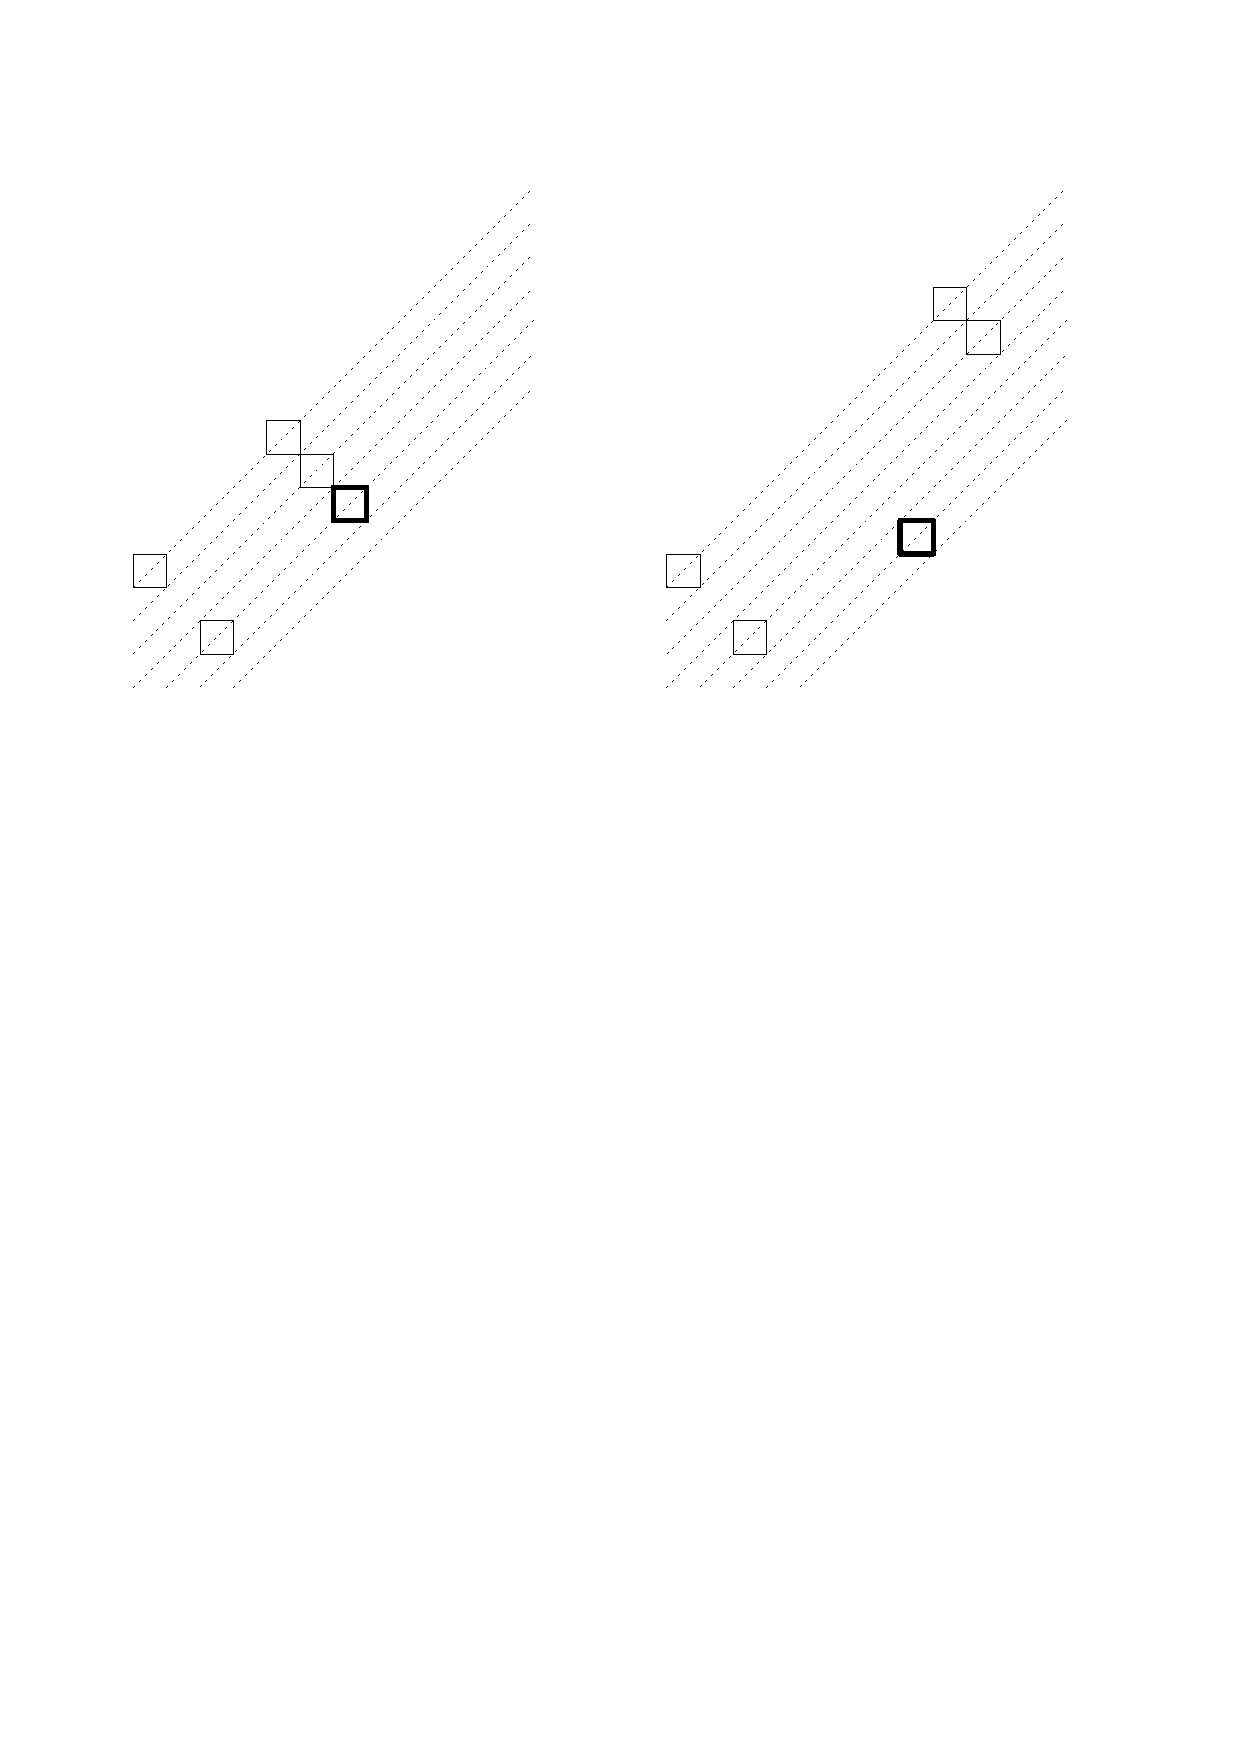
\includegraphics[scale=0.75]{sym/R4-1}
  \end{figure}

\item \textbf{(D2)} If $c(\square_{n-r}) = c(\square_{n}) - 1$, then move
  $\square_{n}$ to immediately after $\beta_{n-r}$ in diagonal $c(\square_{n})$.
  \begin{figure}[H]
    \centering
    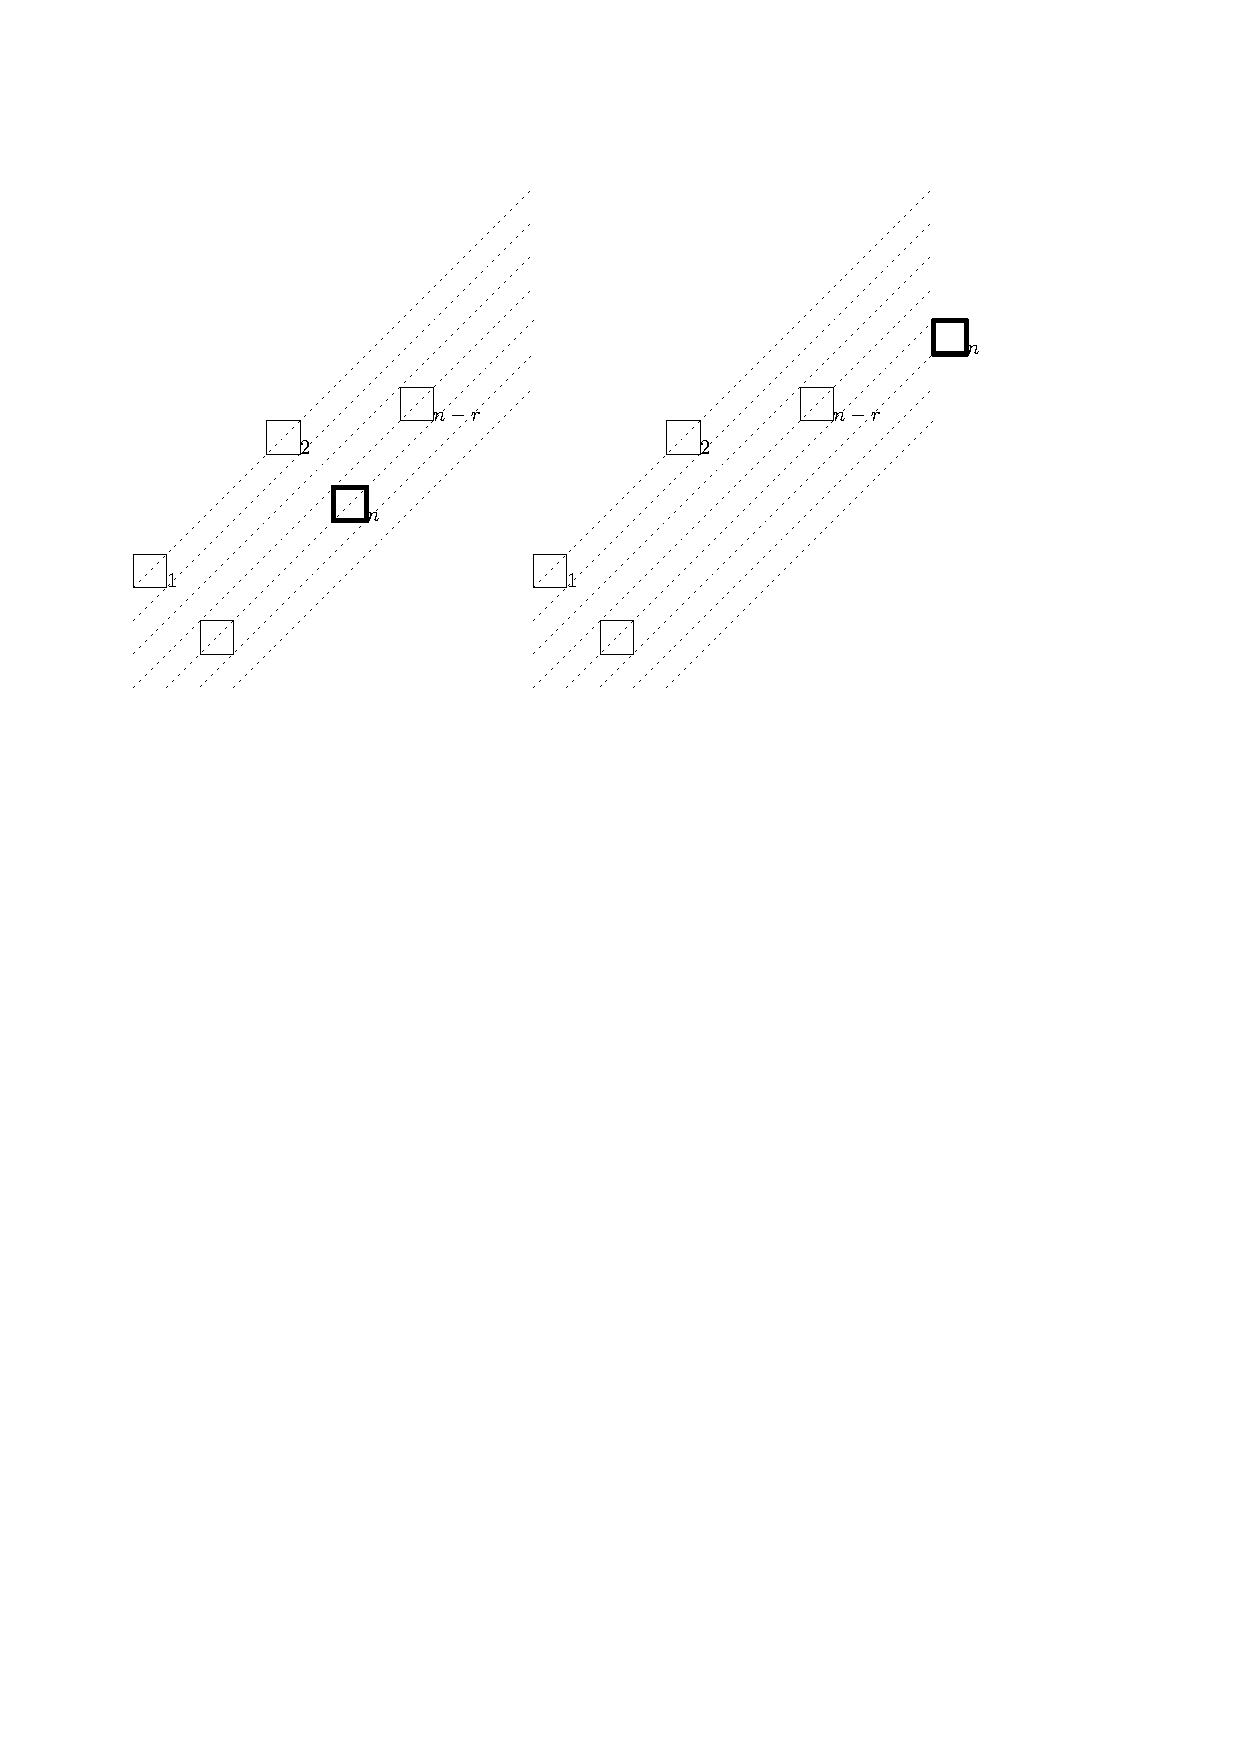
\includegraphics[scale=0.75]{sym/R4-2}
  \end{figure}
\end{itemize}
In either case, the content reading word of the cells do not change.
Denote this new tuple of shapes by $\alpha$ which is still unicellular and
satisfy
\[
  c_{\alpha}(\square_{n-r}) = c_{\alpha}(\square_{n}) - 1 \quad\textrm{and}\quad \square_{n-r} \textrm{
    appears to the left of } \square_{n}.
\]

Note $SSYT(\alpha) \cong SSYT(\beta)$ is simply the set of binary words of length
$n$ under the identification
$T_{\beta}(\square_{i}) = T_{\alpha}(\square_{i}) = w_{i}$ for every
$w \in \{1,2\}^{n}$.  Furthermore,
\[
  inv_{\alpha}(w) =
  \begin{cases}
    inv_{\beta}(w) - 1, &\textrm{if } w_{n-r} = 2 \textrm{ and } w_{n} = 1, \\
    inv_{\beta}(w), &\textrm{otherwise}.
  \end{cases}
\]

Let $\gamma = \beta \setminus \{\square_{n-r},\square_{n}\} = \alpha \setminus \{\square_{n-r},\square_{n}\}$. Then
\[
  G_{\beta}(x_{1},x_{2}; q) - G_{a}(x_{1}, x_{2}; q) = (q^{r} - q^{r-1})
  x_{1}x_{2} G_{\gamma}(x_{1},x_{2};q).
\]
By induction on $r$, we get $G_{\alpha}$ is symmetric.  By induction on
$n$, we get $G_{\gamma}$ is symmetric.

\subsubsection{$\omega$-action via ``superization''}

\subsubsection{Towards A Combinatorial Proof}

We can assume that $\nu$ has no empty diagonals.

\subsection{Connections}
\label{sec:connections}

Elementaries $e_{\lambda}$ can also be thought of a vertical strip Schur
functions whose strips are $\lambda_{1}, \dots, \lambda_{\ell}$ shifted at the correct
height.  From this point of view, the elementaries are not that
different from ribbon Schur functions: We get ribbons by simply shifts
some boxes up and subtract a bunch terms.  But $e_{\lambda}$ can also be
thought of vertical strip LLTs at $q=1$ and ribbons can be thought of
LLTs at $q=0$.  Does this mean we can obtain an interpolation between
$e_{\lambda}$ and ribbons?

Modified Macdonald polynomials.

Parking function characteristic polynomials.

\subsection{Other Conventions}

%%% Local Variables:
%%% mode: latex
%%% TeX-master: "../notes"
%%% End:
